\documentclass{beamer}
\mode<presentation>


\usepackage[brazil]{babel}
\usepackage[utf8]{inputenc}
 


\usepackage{amsfonts}
\usepackage{amssymb}
\usepackage{amsmath}
\usepackage{algorithm}
\usepackage{algpseudocode}



\usepackage{ae}
\usepackage{graphicx,color}
\usepackage[all]{xy}
\usepackage{empheq}
\usepackage{fancybox}
\usepackage{textcomp}
\usepackage[all]{xy}
\usepackage{textpos}
\usepackage{multicol}
\usepackage{cancel}
\usepackage{listings}
\usepackage{xcolor}
\usepackage{enumerate}
\usepackage{minted}

\usepackage[style=verbose]{biblatex}
\addbibresource{bibtex.bib}

\usepackage{tikz}
\usetikzlibrary{shapes.geometric, arrows}


\tikzstyle{startstop} = [rectangle, rounded corners, minimum width=3cm, minimum 
\tikzstyle{io} = [trapezium, trapezium left angle=70, trapezium right angle=110, minimum width=3cm, minimum height=1cm, text centered, draw=black, fill=blue!30]
\tikzstyle{process} = [rectangle, minimum width=3cm, minimum height=1cm, text centered, draw=black, fill=orange!30]
\tikzstyle{decision} = [diamond, minimum width=3cm, minimum height=1cm, text centered, draw=black, fill=green!30]
\tikzstyle{arrow} = [thick,->,>=stealth]

\newcommand{\floor}[1]{$\lfloor$ #1 $\rfloor$}

\newcommand\Fontvi{\fontsize{9}{7.2}\selectfont}



\usetheme{Boadilla}

\newcommand{\PC}[1]{\ensuremath{\left(#1\right)}}


\newcommand*{\colorboxed}{}
\def\colorboxed#1#{%
  \colorboxedAux{#1}%
}
\newcommand*{\colorboxedAux}[3]{%
  % #1: optional argument for color model
  % #2: color specification
  % #3: formula
  \begingroup
    \colorlet{cb@saved}{.}%
    \color#1{#2}%
    \boxed{%
      \color{cb@saved}%
      #3%
    }%
  \endgroup
}



\title {Pensando Computacionalmente}

\author[Wladimir Araújo Tavares]{ Wladimir Araújo Tavares$^{1}$  }

\institute[UFC]{$^{1}$Universidade Federal do Ceará - Campus de Quixadá\\}
\date{}
\AtBeginSection[]
{
  \begin{frame}<beamer>{}
    \small
    \tableofcontents[currentsection,currentsubsection]
  \end{frame}
}
\begin{document}

\begin{frame}
	\titlepage
\end{frame}

%%%%%%%%%%%%%%%%%%%%%%%%%%%%%%%%%%%%%%%%%%%%%%%%%%%%%%%%%%%%%%%%%%%%



\begin{frame}{Multiplicação Egípcias}

\begin{itemize}
\item \textbf{Objetivos:} Desenvolver o pensamento algorítmico

\item \textbf{Público-alvo:}  Alunos a partir do primeiro ano do Ensino Médio.

\item \textbf{Conteúdo:} Algoritmo, Recorrência

\item \textbf{Tempo:} 50 minutos

\item \textbf{Recursos:} Papel, Caneta.

\end{itemize}
    
\end{frame}


\begin{frame}{Passo 1 - Apresentação da Atividade}

\begin{itemize}
   
\item <1-> O método de multiplicação egípcia está descrito no papiro de Rhind datado de 1650 A.C. 

\item Neste método, a multiplicação de dois números é realizado usando apenas a operação de multiplicação por 2, divisão por 2 e soma.



\end{itemize}

\end{frame}


\begin{frame}{Passo 1 - Apresentação da Atividade}

\begin{itemize}
    
    
    \begin{block}{Método de Ahmes}
    O produto de dois números $a$ e $b$, denotado por $a \times b$, pode ser calculado pelas seguintes regras:
    
    \begin{enumerate}
        \item Se $a = 1$, $a \times b = b$.
        \item Se $a$ é par então $a \times b = (a/2) \times (2b)$.
        \item Se $a$ é ímpar maior que 1 então $a \times b = ((a-1)/2) \times (2b) + b$.
        
    \end{enumerate}
    
    \end{block}
    
    \item Neste método, estamos reduzindo o primeiro fator da multiplicação até chegar um caso bem pequeno.
    
\end{itemize}
    
    
\end{frame}


\begin{frame}{Passo 1 - Apresentação da Atividade}


    \begin{block}{Método de Ahmes}
    Calculando $6 \times 7$
    
    \begin{itemize}
        \item Passo 1: Como 6 é par, então $6 \times 7 = 3 \times 14$
        \item Passo 2: Como 3 é ímpar, então $3 \times 14 =  (3-1)/2 \times 28 + 14$
        \item Passo 3: $1 \times 28 + 14 = 42$
    \end{itemize}
    
    \end{block}
\end{frame}



\begin{frame}{Passo 1 - Apresentação da atividade}

Uma maneira mais fácil de utilizar o método de multiplicação egípcia é utilizando uma tabela com duas colunas. Quando o número da primeira coluna for ímpar, somamos os valores da segunda coluna.

    \begin{block}{Método de Ahmes}
    Calculando $6 \times 7$
    
    \begin{center}
    \begin{tabular}{c|c|c}
    a & b & a é par\\
    \hline
    6 & 7 & sim\\
    3 & 14 & não\\
    1 & 28 & não\\
    \end{tabular}
    \end{center}
    
    Podemos observar que toda vez que a é ímpar, uma parcela com valor b é adicionado ao resultado. Logo, $6 \times 7 = 14 + 28 = 42.$
    
    \end{block}
\end{frame}




\begin{frame}{Passo 2 - Execução da atividade}

Os alunos devem realizar as seguintes multiplicações utilizando o método egípcio:

\begin{enumerate}
    \item $35  \times 14$
    \item $40  \times 63$
    \item $45  \times 63$
\end{enumerate}





\end{frame}



\begin{frame}{Passo 3 - Fluxograma}



\begin{center}
	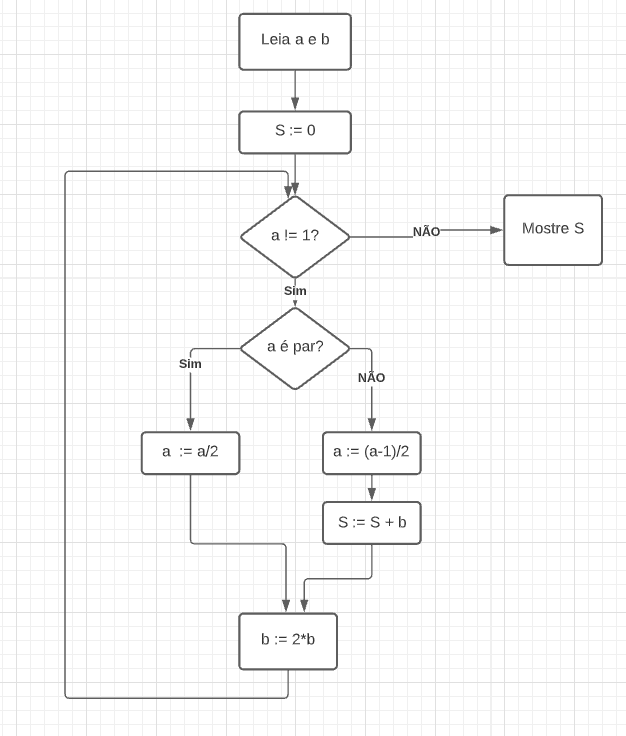
\includegraphics[scale=0.3]{images/fluxograma.png} 
\end{center}






\end{frame}


\begin{frame}{Passo 4 - Comandos no Scratch}



\begin{center}
	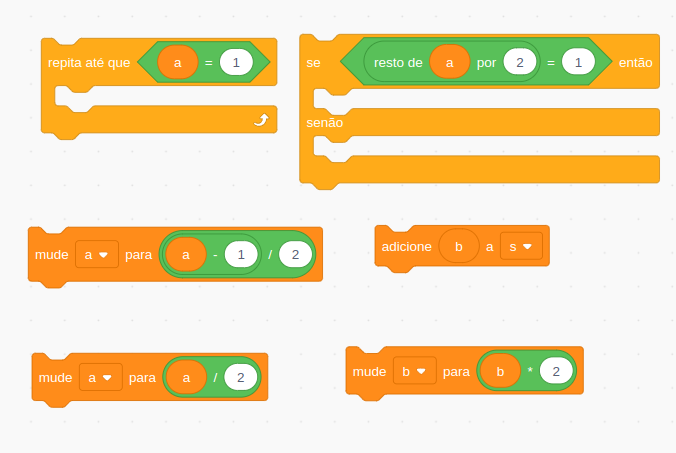
\includegraphics[scale=0.5]{images/multiplicacao egípcia.png} 
\end{center}

\end{frame}

\begin{frame}{Passo 5 - Programando no Scratch}



\begin{center}
	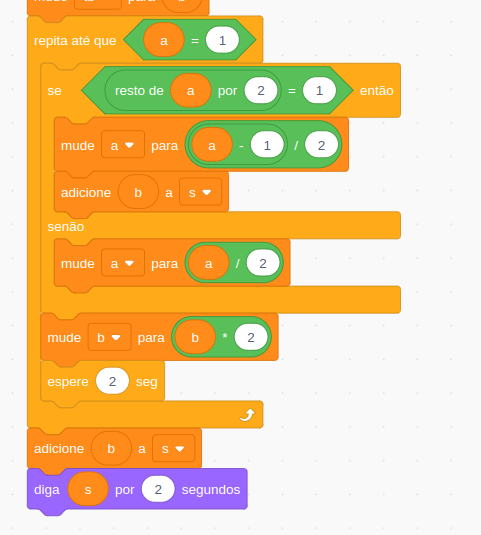
\includegraphics[scale=0.4]{images/scratch.png} 
\end{center}



\end{frame}


\begin{frame}{Passo 6 - Discussão e Avaliação}

\begin{itemize}

\item<1-> Os alunos são incentivados a escrever sobre as dificuldades para realizar o procedimento.

\item<2-> Quais são as vantagens de utilização deste método?


\end{itemize}


\end{frame}





\end{document}